\Askhsh{33628}{4}
\begin{ylh}{1}
    \item 1.1 Συναρτήσεις.
    \item 1.3 Παράγωγος συνάρτησης.
    \item 1.4 Εφαρμογές των Παραγώγων.
\end{ylh}
\begin{wrapfigure}[9]{r}{5cm}
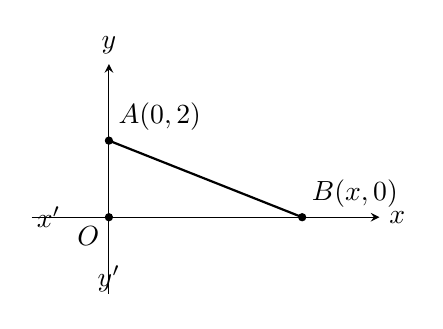
\begin{tikzpicture}[scale=1]
\begin{axis}[
    axis lines=middle,
    xmin=-2, xmax=7,
    ymin=-2, ymax=4,
    xtick=\empty,
    ytick=\empty,
    xlabel=$x$,
    ylabel=$y$,
    every axis x label/.style={at={(current axis.right of origin)}, anchor=west},
    every axis y label/.style={at={(current axis.above origin)}, anchor=south},
    width=6cm, height=4.5cm,
    clip=false
]
    % Draw segment AB
    \draw[thick] (axis cs:0,2) -- (axis cs:5,0);
    
    % Plot points A, B and Origin O
    \fill (axis cs:0,2) circle (1.5pt) node[anchor=south west] {$A(0,2)$};
    \fill (axis cs:5,0) circle (1.5pt) node[anchor=south west] {$B(x,0)$};
    \fill (axis cs:0,0) circle (1.5pt) node[anchor=north east] {$O$};
    
    % Add labels for x' and y'
    \node at (axis cs:-1, 0) [anchor=east] {$x'$};
    \node at (axis cs:0, -1) [anchor=north] {$y'$};
\end{axis}
\end{tikzpicture}
\end{wrapfigure}
Στο παρακάτω σχήμα δίνονται τα σημεία $A(0,2)$ και $B(x,0)$ με $x>0$.

\begin{alist}
\item Να δείξετε ότι η απόσταση των σημείων $A$ και $B$ συναρτήσει του $x$ είναι:
\[ d(x) = (\mathrm{AB}) = \sqrt{x^2+4} \text{ με } x>0. \]
\monades{8}

\item Να βρείτε το ρυθμό μεταβολής της απόστασης των σημείων $A$ και $B$ ως προς $x$ όταν $x=3$.
\monades{9}

\item Ένας μαθητής παρατήρησε ότι, καθώς το σημείο $B$ κινείται προς τα δεξιά στον ημιάξονα $Ox$, το μήκος του $AB$ αυξάνεται. Να αιτιολογήσετε γιατί συμβαίνει αυτό, αξιοποιώντας το ερώτημα (β).
\monades{8}
\end{alist}

